We will first define timed automata and zones, a method used to represent time in timed automata. Also a subsumption check over zones will be defined. 

\subsection{Timed Automata}
Timed automata is a formalism that extends labelled transition systems with one or more clocks. Guards over these clocks, denoted as $G(C)$ can be used for transitions and as invariants. 

\begin{mydef}[Clock Guards]
\label{def:clockGuards}
$G(C)$ is the set of conjunctions over simple conditions of the form $x \Join c$ or $x-y \Join c$, where $x,y \in C$, $c \in \mathbb{N}$ and $\Join \in \{<,\leq,=,\geq,>\}$.
\end{mydef}

Timed automata use a notion of downwards closed clock invariants. We define a downwards closed set and specify this for clock guards.

\begin{mydef}[Downwards Closed Set]
A set $A$ is downwards closed if $\forall a \in A. x \preceq a \implies x \in A$. 
\end{mydef}

For clock guards we define the operator $\preceq$ to be true for $x \Join c \preceq x \Join' c'$ if $c < c'$ or $c = c'$ and $\Join = < \wedge \Join' = \leq$. This leads to a much simpler definition of downwards closed clock guards.

\begin{mydef}[Downwards Closed Clock Guards]
A set $G(C)$ is downwards closed if all simple conditions are of the form $x \Join c$ or $x-y \Join c$, where $x,y \in C$, $c \in \mathbb{N}$ and $\Join \in \{<,\leq\}$.
\end{mydef}


Also reset actions for clock can be defined for transitions, setting clocks to $0$. All clocks in the system will increase at the same rate. As our work continues on~\cite{eemcs21972} we use the same definition of timed automata.

\begin{mydef}[Timed Automata]
\label{def:TA}
An extended timed automaton is a 6-tuple A = $\langle L, C, Act, l_0, \rightarrow, I_c\rangle$ where
{\renewcommand\labelitemi{--}
	\begin{itemize}
		\item L is a finite set of locations, typically denoted by $l$
		\item C is a finite set of clocks, typically denoted by c
		\item Act is a finite set of actions
		\item $l_0 \in$ L is the initial location
		\item $\rightarrow \subseteq L \times G(C) \times Act \times 2^C \times L$ is the (non-deterministic) transition relation. We normally write l $\stackrel{g,a,r}{\longrightarrow}$ l' for a transition., where l is the source location, g is the guard over the clocks, a is the action, and r is the set of clocks reset.
		\item $I_C : L \rightarrow G(C)$ is a function mapping locations to downwards closed clock invariants.
	\end{itemize}
}
\end{mydef}

In the rest of this thesis we will not strictly stick to the definition of locations. We use the terminology 'locations' and other 'discrete variables'. Locations are the locations in the \uppaal{} transition system editor, the other discrete variables are declared in the C-like syntax that \uppaal{} uses. With the definition of a timed automaton we can combine a finite number of timed automata to a network of timed automata, which is a parallel composition, to define larger systems. This is a parallel composition that synchronizes on a set of channels $Chan$~\cite{UPPAAL}. $ch!$ and $ch?$ represent the output and input action on the channel $ch \in Chan$.

\begin{mydef}[Network of timed automata~\cite{eemcs21972}]
\label{def:networkTA}
Let Act = $\{ch!,ch?|ch \in Chan\} \cup \{\tau\}$ be a finite set of actions, and let C be a finite set of clocks. Then the parallel composition of extended timed automata $A_i = \langle L_i, C, Act, l^i_0, \rightarrow_{i}, I^i_C\rangle$ for all $1 \leq i \leq n$, where $n \in \mathbb{N}$, is a network of timed automata, denoted $A = A_1||A_2||..||A_n$.
\end{mydef}

\subsection{Zones}
For basic transition systems the state space can grow exponentially for the number of variables in the system. The state space of timed automata is by definition infinite, as clocks have real values. If a discrete state is defined between two points in time, an infinite amount of moments in time can happen during that state. Even when some granularity is used, that defines that clocks will only increase with certain step size the automata can still have infinite state space if a clock is unbounded. To tackle this problem most model checkers use a notion of zones for the representation of time. A zone can be seen as a set of clock guards. To represent these zones several data structures have been developed. One of the most common used structures are Difference Bound Matrices (DBMs)~\cite{dbmorig,bengtsson2002clocks}.

\begin{mydef}[Difference Bound Matrix]
A DBM for the clocks $C = \{c_1,...c_n\}$ is a $(n+1)^2$ matrix. Each position has the following attributes.

\begin{tabular}{lll}
Attribute                & Type                      & Description                                           \\\hline
const(i,j)               & $\mathbb{Z}$             & Constant value $c$ \\
op(v)                    & \{$<$, $\leq\}$     & Operator $<$ or $\leq$.                         \\
\end{tabular}

Each position $(i,j)$ defines an upper bound on the value of $c_i - c_j$. On the first row and first column an extra clock $\mathbf{O}$ is added as $c_0$ with constant value 0. 
\end{mydef}
 
These matrices use both a column and a row for each clock, and on each position $(i,j)$ an upper bound on the difference between the clocks $c_i$ and $c_j$ is given in the form $c_i - c_j \preceq x$ where $\preceq \in \{<, \leq\}$ and $x \in \mathbb{Z}$. For the constraints over the single clocks an extra clock $\mathbf{O}$ with a constant value 0 is added. This way the upper and lower bound of a clock $c_i$ can be given by $c_i - \mathbf{O} \preceq x$ and $\mathbf{O} - c_i \preceq y$. The addition of this $\mathbf{O}$ clock will give the matrix of a timed automaton always size $(|C|+1)^2$. This way convex zones of clock variables can be represented. Each matrix can however only contain a single convex zone. Concave zones and multiple convex zones need multiple matrices to be represented. As a solution often a list of DBMs is used. In figure \ref{fig:dbm} we give an example of a DBM with two clocks: $c_1$ and $c_2$, representing the zone $0 \leq c_1 < 5 \wedge 0 \leq c_2 \leq 4$. The diagonal only contains $(0,\leq)$ values as these elements give the difference between a clock and itself, which is clearly always 0.

\begin{figure}
	\centering
	\begin{math}
% 		\begin{pmatrix}
 \bordermatrix{ 		                 & \mathbf{O} & c_1           & c_2        \cr
 			\mathbf{O} &(0,\leq)      & (0,\leq)      & (0,\leq)     \cr
 			c_1        &(5,<   )      & (0,\leq)      & (\infty,\leq)\cr
 			c_2        &(4,\leq)      & (\infty,\leq) & (0,\leq)     \cr}
% 		\end{pmatrix}
	\end{math}
	\caption{DBM}
	\label{fig:dbm}
\end{figure}

A number of operations on DBMs has been defined. We will introduce the operations we use. The same notation as~\cite{eemcs21972} is used.
\begin{itemize}
\item $D \uparrow$ is called the delay operator. This lets time pass unlimitedly from the zone in D.
\item $D \cap D'$ adds additional constraints from $D'$ to $D$. This is used for transitions that have clock constraints. These constraints can be represented as a DBM.
\item $D[r]$ with $r \subseteq C$, resets all clocks in $r$.
\item $D/B$ does a maximal bounds extrapolation. In section \ref{subsec:extrapolation} we will go into more detail about this extrapolation.

\end{itemize}

\subsection{Zone subsumption}
\label{subsec:subsumtion}
In model checking an important function is to check if a certain state has been visited already earlier. For normal automata this can be done by comparing the newly found state to all states that have already been visited, and check if one of those states is equal to that new state. This is often done by more efficient methods, like hash functions, but the equality check remains. For states with zones this equality check does not suffice. Two zones do not need to be equal, but the newly discovered zone can also be a subset of the earlier discovered zones. In \ltsmin{} this is done by a subsumption check~\cite{eemcs21972} that is performed over the DBMs. This check is delegated to the \uppaal{} DBM library. The function checks if a new zone is a subset of the zone represented by a DBM.

\subsection{Binary Decision Diagram}
We shortly introduce binary decision diagrams(BDDs)~\cite{Bryant:1986:GAB:6432.6433}. BDDs are the basis of most symbolic model checking techniques. BDDs are a way to represent boolean functions. All diagrams that we discuss in the rest of this thesis are based on BDDs.
\begin{figure}[h]
\centering
	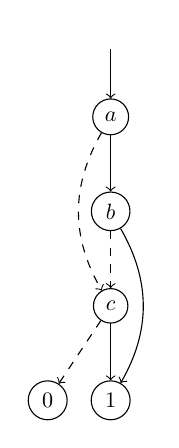
\begin{tikzpicture}[
		smallvertex/.style={circle,draw,scale=0.8}
		]
		\node[smallvertex](S1){$a$};
		\node[smallvertex, draw = none, above of = S1, yshift = 0.25cm](S0){};
		
		\node[smallvertex, below of = S1, yshift = -.5cm](S2){$b$};
		\node[smallvertex, below of = S2, yshift = -.5cm](S3){$c$};
		\node[smallvertex, below of = S3, yshift = -.5cm](S4){$1$};
		\node[smallvertex, left of = S4](S5){$0$};
		
		\draw[->] (S0) --(S1) node [midway, above, sloped, scale=0.75,
		rotate=0, xshift =-0.4 cm, yshift = -0.2cm]{};
		\draw[->] (S1) --(S2) node [midway, above, sloped, scale=0.75,
		rotate=90, xshift =-0.4 cm, yshift = -0.2cm]{};
		\draw[dashed,->] (S2) --(S3) node [midway, above, sloped, scale=0.75,
		rotate=90, xshift =-0.4 cm, yshift = -0.2cm]{};
		\draw[->] (S3) --(S4) node [midway, above, sloped, scale=0.75,
		rotate=90, xshift =-0.4 cm, yshift = -0.2cm]{};		
		\draw[->,dashed] (S1) edge[bend right](S3) node [midway, above, sloped, scale=0.75,
		rotate=90, xshift =-0.4 cm, yshift = -0.2cm]{};	
		\draw[->] (S2) edge[bend left](S4) node [midway, above, sloped, scale=0.75,
		rotate=90, xshift =-0.4 cm, yshift = -0.2cm]{};	
		\draw[dashed,->] (S3) --(S5) node [midway, above, sloped, scale=0.75,
		rotate=90, xshift =-0.4 cm, yshift = -0.2cm]{};
		[bend left]
	\end{tikzpicture}
\caption{A BDD representing $(a \wedge b) \vee c$}
\label{fig:BDD}
\end{figure}



\begin{mydef}[Binary Decision Diagram~\cite{Bryant:1986:GAB:6432.6433}]
A BDD is a rooted, directed graph with vertex set $V$ containing two types of vertices. A nonterminal vertex $v$ has as attributes an argument index $index(v) \in \{1,...,n\}$, and two children $low(v),high(v) \in V$. A terminal vertex $v$ has as attribute a value $value(v) \in \{0,1\}$
\end{mydef}



\begin{mydef}[BDD Semantics~\cite{Bryant:1986:GAB:6432.6433}]
A BDD $G$ having root vertex $v$ denotes a function $f_v$ defined recursively as:
\begin{itemize}
\item If $v$ is a terminal vertex:
\begin{itemize}
\item If $value(v)=1$, then $f_v=1$
\item If $value(v)=0$, then $f_v=0$
\end{itemize}
\item If $v$ is a nonterminal vertex with $index(v)=i$ then $f_v$ is the function
$f_v(x_1,...,x_n) = \overline{x_i}\cdot f_{low(v)}(x_1,...,x_n)+x_i\cdot f_{high(v)}(x_1,...,x_n)$.
\end{itemize}
\end{mydef}

The high and low edges of a node are graphically shown as a straight and a dotted line respectively. A BDD can also be reduced and ordered, we will not go into detail on that here. In Figure \ref{fig:BDD} we show a BDD representing the boolean formula $(a \wedge b) \vee c$. For larger diagrams, edges that go directly to the terminal vertex with value $0$ are often omitted for better readability. 